

    \item A symmetric star shaped conducting wire loop is carrying a steady state current \( I \) as shown in the figure. The distance between the diametrically opposite vertices of the star is \( 4a \). The magnitude of the magnetic field at the center of the loop is
        \begin{tasks}(2)
            \task \(\frac{\mu_0 I}{4\pi a} [6\sqrt{3} - 1]\)
            \task \(\frac{\mu_0 I}{4\pi a} [6\sqrt{3} + 1]\)
            \task \(\frac{\mu_0 I}{4\pi a} [3\sqrt{3} - 1]\)
            \task \(\frac{\mu_0 I}{4\pi a} [2 - \sqrt{3}]\)
        \end{tasks}

\begin{center}
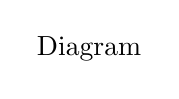
\begin{tikzpicture}
\node {Diagram};
\end{tikzpicture}
\end{center}
